\begin{section}{Resultados}

\subsection{Diagrama do Sistema}

\begin{figure}
    \centering
    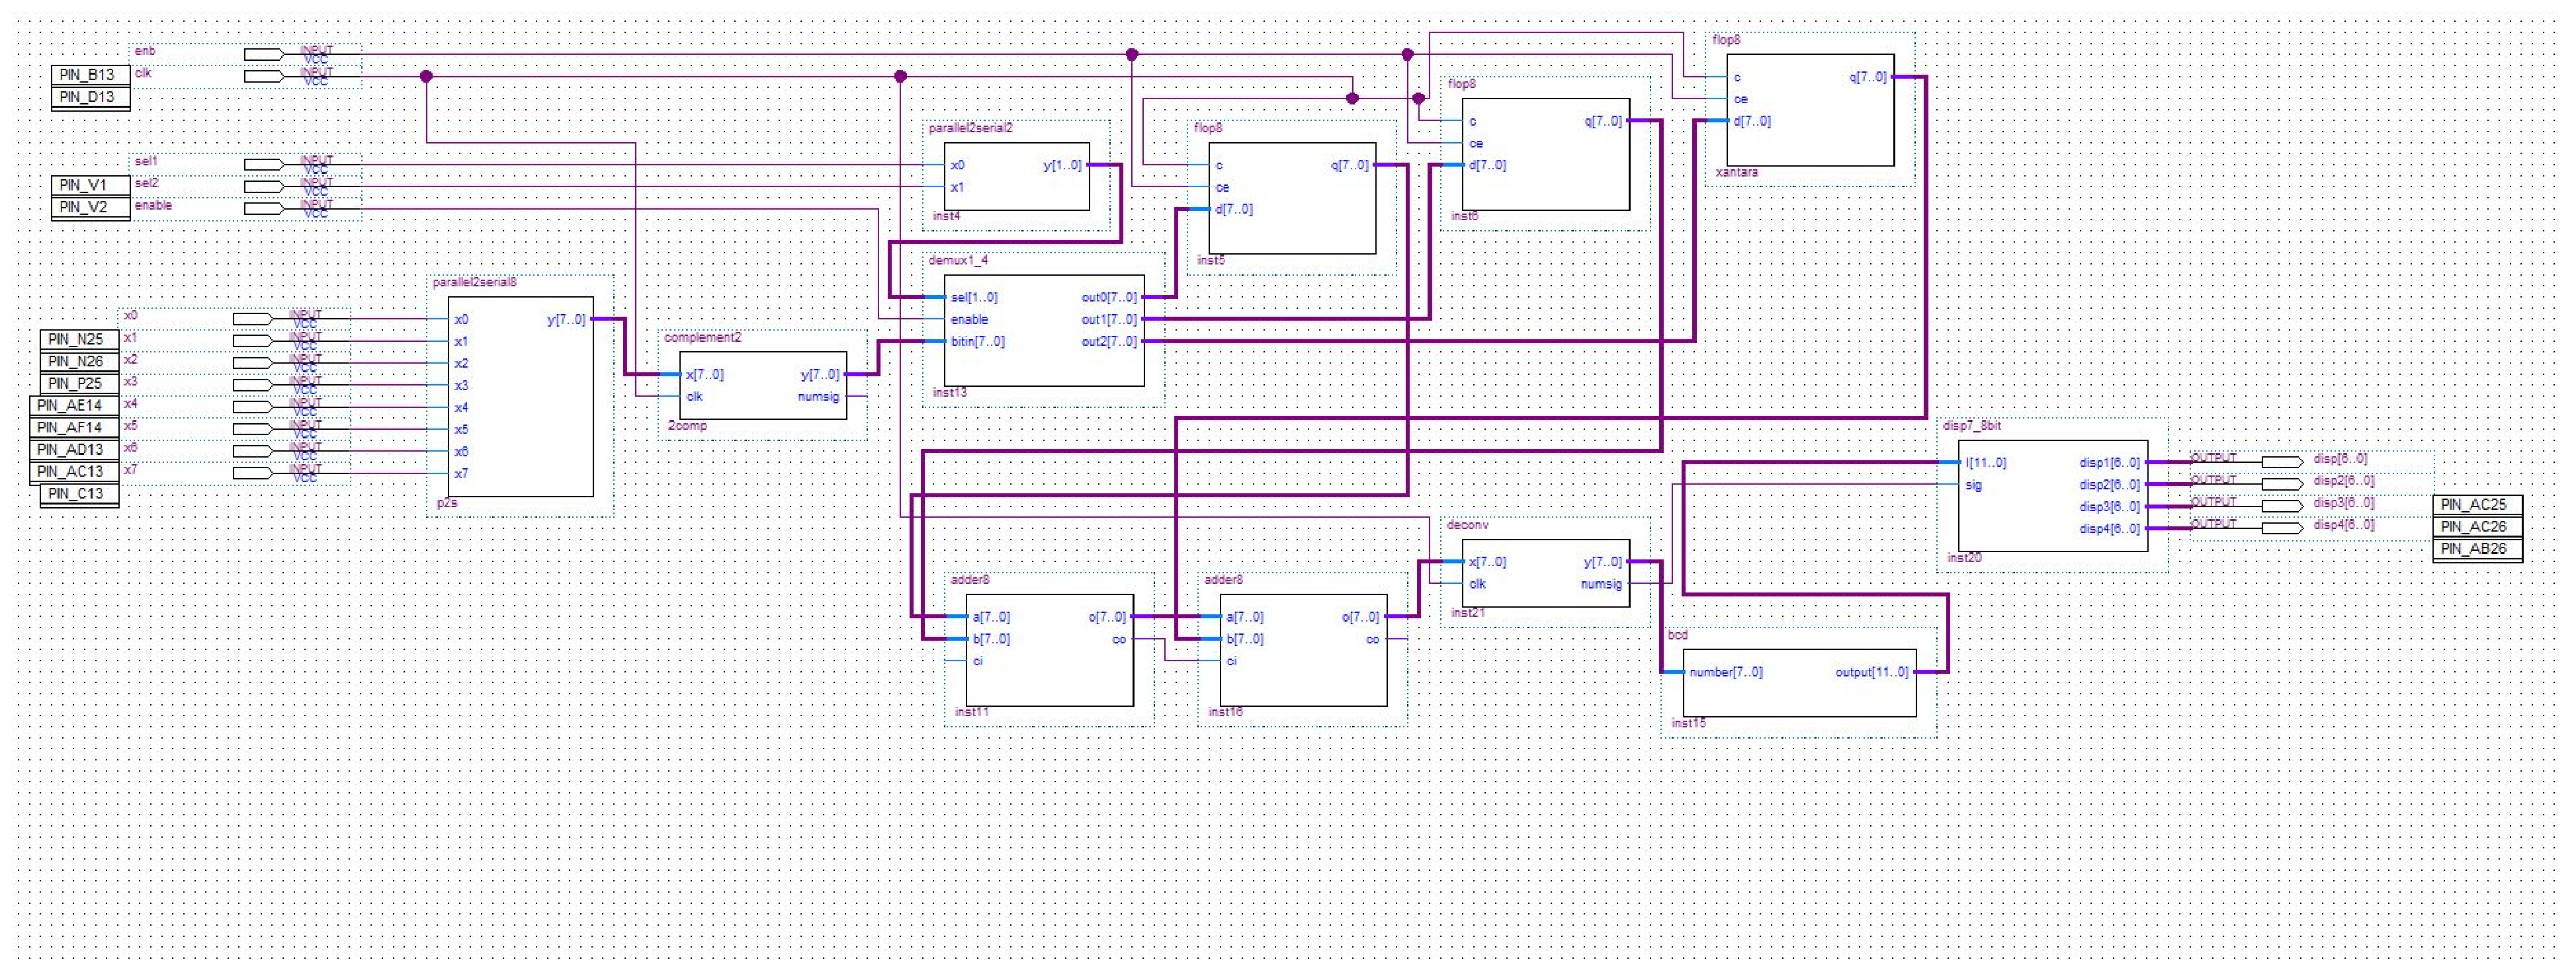
\includegraphics[width=.90\textwidth]{Figures/system_sch}
    \caption{Esquem�tico do Sistema no QuartusII}
    \label{fig:system}
\end{figure}

\subsection{Simula��o}
Todos os blocos do sistema foram devidamente simaulado sno \emph{ModelSim},
muitos por se tratarem de blocos intermedi�rios no sistema, n�o havia muito
sentido em algumas delas.\\
Abaixo � mostrada a sa�da da simula��o do bloco somador:

\begin{figure}
    \centering
    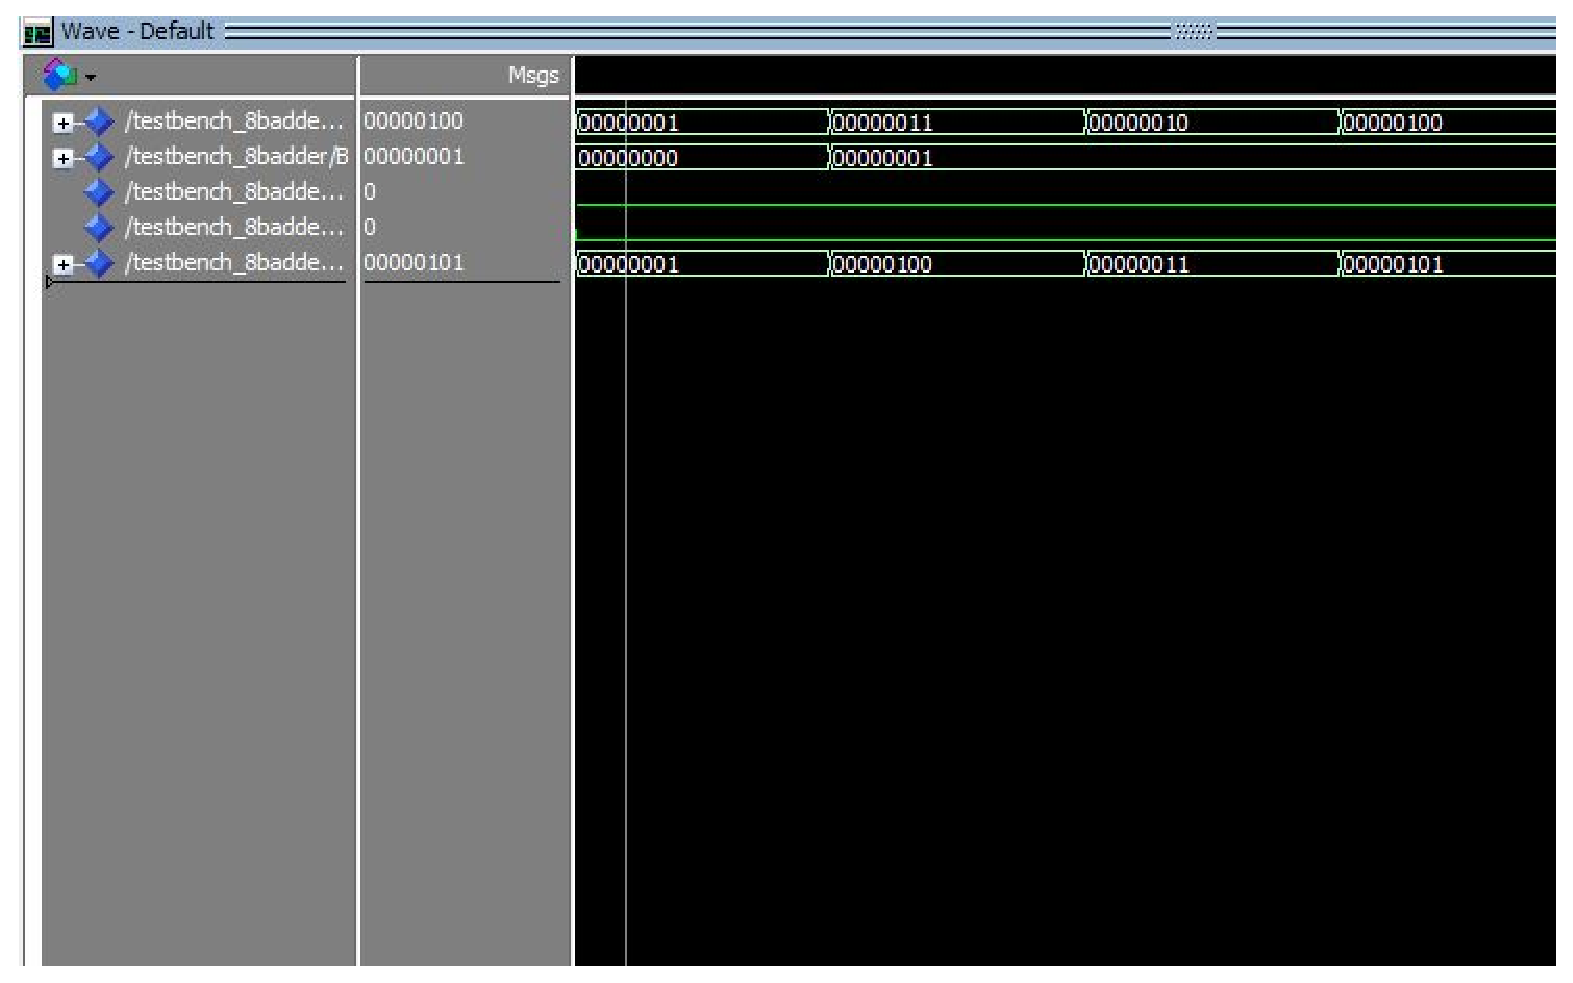
\includegraphics[width=.85\textwidth]{Figures/tb_adder8}
    \caption{Esquem�tico do Sistema no QuartusII}
    \label{fig:system}
\end{figure}

\subsection{Execu��o}
Na finaliza��o do projeto h� alguns pontos a serem salientados.\\

\begin{itemize}
    \item Durante o desenvolvimento do sistema houveram algumas diferen�as na simula��o e
no c�digo que foi mebarcado na fpga, ent�o a partir de certo ponto foi optado o
teste somente na placa.
    \item N�o houve tempo para tratamento de estouro de buffer, ent�o em alguns
        casos a sa�da era o resultado somado com um, o que foi resolvido
        retirando a liga��o entre carry in/carry out do primeiro para o segundo
        somador.
\end{itemize}

\end{section}
%%% EOF %%%
